\documentclass[a4paper, 11pt]{article}

\usepackage[portuges]{babel}
\usepackage[utf8]{inputenc}
\usepackage{amsmath}
\usepackage{indentfirst}
\usepackage[table,xcdraw]{xcolor}
\usepackage{graphicx}
\usepackage{tabto}
\usepackage{float}
\usepackage{adjustbox}
\usepackage[pdftex]{color,graphicx}
\usepackage[left=2cm,top=2.5cm,right=2.5cm,bottom=2.5cm]{geometry}
\usepackage{enumerate}% http://ctan.org/pkg/enumerate
\usepackage{xurl}
\usepackage{hyperref}

\begin{document}
\begin{titlepage}
    \begin{center}

    	
\includegraphics[width=0.3\textwidth]{images/Capa/EEUMfinal .png}
       
       \vspace*{1cm}
       
       \textbf{\Large Engenharia de Serviços em Rede}
        \vspace{1cm}
        \par
        \textbf{\Large Serviço Over the Top para entrega de multimédia}
        \vspace{1cm}
        \par
        \Large \textbf{PL3 - Grupo 5}
        
       Luis Sousa a89597\\Maria Barros pg47488\\Pedro Barbosa pg47577
       \vspace{1cm}
	\begin{figure}[!htb]
	    \hspace{1.5cm}
        \minipage{0.25\textwidth}%
            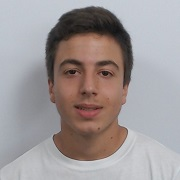
\includegraphics[width=\linewidth]{images/Capa/80.jpg} 
            \centering
            \captionsetup{a89597}
        \endminipage
        \hspace{-0.2cm}
        \minipage{0.25\textwidth}%
            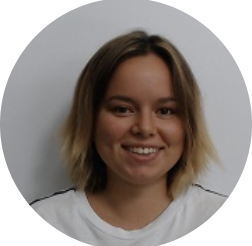
\includegraphics[width=\linewidth]{images/Capa/44.jpg} 
            \centering
            \captionsetup{pg47488}
        \endminipage
        \hspace{-0.2cm}
        \minipage{0.25\textwidth}%
            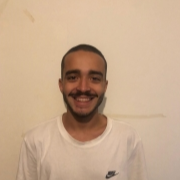
\includegraphics[width=\linewidth]{images/Capa/154.jpg} 
            \centering
            \captionsetup{pg47577}
        \endminipage
    \end{figure}

\blindtext

\vspace{2cm}
        
        29 de dezembro de 2021
            
    \end{center}
\end{titlepage}

\newpage
\tableofcontents
\newpage
\section{Introdução}
Ao longo do último meio século de vida da Internet (a rede das redes), observou-se uma mudança irreversível de paradigma. A comunicação extremo-a-extremo, de sistema final para sistema final, dá lugar ao consumo voraz de conteúdos de qualquer tipo, a todo o instante, em contínuo e muitas vezes em tempo real. Este novo padrão de uso coloca grandes desafios à infraestrutura IP de base que a suporta. Apesar de não ter sido originalmente desenhada com esse requisito, tem sido possível resolver a entrega massiva de conteúdos com redes sofisticadas de entrega de conteúdos (CDNs) e com serviços específicos, desenhados sobre a camada aplicacional, e por isso ditos Over the Top (OTT). \\

Over-the-top é um termo genérico para um serviço utlizado sobre uma rede que não é oferecido pelo operador. É normalmente descrito como "over-the-top", pois estes serviços funcionam sobre um serviço já existente e não requerem qualquer afiliação com tecnologias ou modelos de negócio associadas ao operador de telecomunicaçôes. Pode também ser definido como contéudo multimédia (televisão e conteúdo vídeo, por exemplo) distribuídos através de uma ligação Internet
de alta velocidade e não de um provedor de serviços por cabo ou satélite. 

A aplicação mais comum do modelo OTT é, sem dúvida, no dominio de vídeo digital, onde os fornecedores de conteúdo dependem de um operador de telecomunicações para disponibilizar conteúdo (muitas vezes interativo) para televisões, box por cabo e computadores pessoais. \cite{ott}\\

Um serviço de multimedia OTT, pode por exemplo usar uma rede overlay aplicacional, devidamente configurada e gerida para contornar os problemas de congestão e limitação de recursos da rede de suporte, entregando em tempo real e sem perda de qualidade os videos diretamente ao cliente final.
Para tal, formam uma rede overlay própria, assente em cima dos protocolos de transporte (TCP ou UDP) e/ou aplicacionais (HTTP) da Internet. Neste trabalho pretende-se conceber e prototipar um desses serviços, que promova a eficiência e a otimização de recursos para melhor qualidade de experiência do utilizador. 


%-----------------------------------------------------------%


\section{Arquitetura da solução}

\begin{figure}[h]
    \centering
    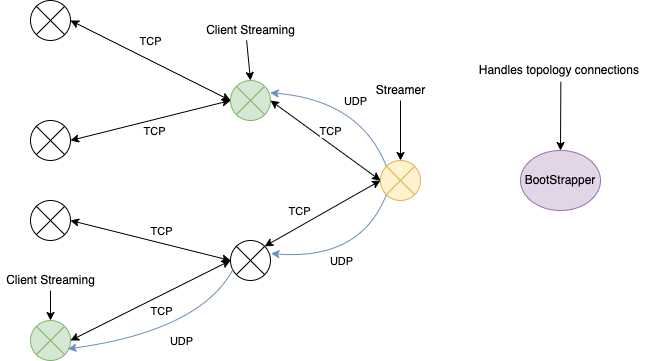
\includegraphics[height=0.5\textwidth, width=0.9\linewidth]{images/redesnacho.png}
    \caption {Diagrama : Arquitetura do Sistema}
\end{figure} 

\newpage

Inicialmente, começamos por definir qual a linguagem de programação que iremos usar para desenvolver o projeto. Assim, chegando a um consenso, escolhemos Java. Para além de já termos feito bastantes projetos com esta mesma linguagem, o que nos facilitará em algumas partes do trabalho, acreditamos que Java seja a linguagem mais apropriada para termos uma boa prestação neste trabalho prático.\\ 

Posteriormente, surgiu-nos um desafio de definir que protocolos iremos utilizar ao longo do projeto. Assim sendo, debatemos entre os elementos do grupo, e chegamos à conclusão que iremos utilizar o protocolo \textit{TCP} para a construção da rede, isto é, construção das conexões entre nodos e servidor e envio de algumas mensagens entre eles. Para a parte restante do trabalho, ou seja, etapa em que iremos nos preocupar com streaming de video iremos usar protocolos \textit{UDP}.\\

Seguidamente, o nosso grupo pensou na estratégia a utilizar na etapa 1 referente à construção da topologia overlay. Deste modo, decidimos escolher a segunda estratégia que consiste na conceção de um \textit{bootstrapper} que irá controlar toda esta construção. Assim, este lê um ficheiro \textit{.txt} com a configuração da topologia e, a partir do mesmo,  trata das conexões para a construção da mesma. Desta forma, foi criado um \textit{BootstrapperListener} que recebe a lista de nodos necessários para a criação da topologia e cria uma \textit{thread} para cada um deles que vai indicar a cada nodo quantos vizinhos o mesmo possui e quais os seus ips. Em relação à conexão em si, cada nodo irá tentar estabelecer uma com os seus vizinhos. Caso consiga, a conexão estabelecida entre eles é do tipo \textit{TCP}. Aquando da criação de um nodo é também criada uma \textit{thread}, \textit{OttNodeListener}, que estará sempre à espera dos vizinhos que ainda não se conectaram e que o queiram fazer.\\

O próximo passo consistiu na construção das rotas para os fluxos. Começamos por escolher o número de saltos como tipo de métrica para a escolha do melhor caminho. Seguidamente, pensamos sobre este passo e decidimos adotar a primeira estratégia. Sendo a topologia toda construída, o \textit{bootstrapper} avisa o \textit{streamer} que isso aconteceu. De seguida, este irá enviar um \textit{packet} para os seus vizinhos com o número de saltos a 1. Quando cada nodo recebe este \textit{packet} se este número de saltos for menor que o número de saltos do nodo, este irá mudar o seu número de saltos para esse novo número e irá retransmitir o \textit{packet} para os seus vizinhos, e assim sucessivamente. Caso contrário, irá apenas descartar o \textit{packet}.\\

Para a quarta e última etapa escolhemos a primeira estratégia. Desta forma, o \textit{streamer} começa a enviar frame a frame o vídeo que pretende \textit{streamar} encapsulado num \textit{rtpPacket} que, por sua vez, é encapsulado num \textit{DatagramPacket} e envia-o para o/os nodo/os vizinho/os consoante as melhores rotas escolhidas através da etapa anterior. Estes vizinhos voltam a retransmitir o packet para outros vizinhos da mesma forma. Caso queiram consumir a \textit{stream} irão desencapsular os packets e transmitir frame a frame a mesma.


%-----------------------------------------------------------%


\section{Especificação dos protocolos}

\subsection{Formato das mensagens protocolares}

O tipo de mensagens protocolares do nosso projeto difere com o tipo de \textit{packet} utilizado. Existem quatro tipos diferentes:

\begin{itemize}
    \item \textbf{\textit{Packet.START\_FLOODING}}
    
    Este \textit{packet} é enviado pelo \textit{bootstrapper} ao \textit{streamer} em específico, no final da construção da topologia, de modo a este saber que pode iniciar o \textit{flooding}.
    
    \item \textbf{\textit{Packet.FLOODING}}
    
    Este \textit{packet} é enviado de nodo em nodo aquando do \textit{flooding}. Um dos campos deste \textit{packet} é uma mensagem que contém o número de saltos.
    
    \item \textbf{\textit{Packet.CANCEL\_STREAM\_FLOW}}
    
    Este \textit{packet} é enviado aquando do \textit{flooding} para um nodo avisando-o do redirecionamento da \textit{stream} e que esta já não passar por lá.
    
    \item \textbf{\textit{Packet.CONFIRM\_STREAM\_FLOW}}
    
    Este \textit{packet} é enviado aquando do \textit{flooding} para um nodo avisando-o do redirecionamento da \textit{stream} e que esta começa a passar por lá. 
    
\end{itemize}

\subsection{Interações}

Existem as seguintes interações no serviço OTT para entrega de multimédia:

\begin{itemize}
    \item \textbf{\textit{Bootstrapper}-\textit{Streamer}}
    
    No final da construção da topologia avisa o \textit{streamer} que este pode iniciar o \textit{flooding}.
    
    \item \textbf{\textit{Bootstrapper}-\textit{Nodo OTT}}
    
    Interage com o Nodo OTT para a inicialização de conexão entre eles e outros Nodos OTT.
    
    \item \textbf{\textit{Nodo OTT} - \textit{Nodo OTT}}
    
    Interagem entre si tanto para a transmissão de \textit{packets} de \textit{flooding} como para a retransmissão de \textit{packets} de \textit{streaming}.
    
\end{itemize}


%-----------------------------------------------------------%


\section{Implementação}

\subsection{\textit{Package Bootstrapper}}

Este \textit{Package} contém as classes referentes ao \textit{Bootstrapper}.

\begin{itemize}

    \item \textbf{Classe \textit{Bootstrapper}}
    
    Esta classe tem como atributos o \textit{IP} do \textit{Bootstrapper}, a porta pela qual este vai comunicar e uma \textit{string} que é o ficheiro de configuração da topologia. Esta classe espera pela conexão de todos os nodos necessários para arrancar a topologia. Quando isto acontece, é chamada a função \textit{start\_flooding}, que envia um \textit{packet} ao \textit{streamer} para este iniciar o \textit{flooding}.

    \item \textbf{Classe \textit{Topology}}
    
    Esta classe tem como atributos um \textit{Map} que associa um nome de um nodo a uma lista de IPs dos seus vizinhos e uma lista com os nomes dos nodos necessários para a criação da topologia. Nesta classe é feito o \textit{parsing} do ficheiro de configuração da topologia.
    
\end{itemize}

\subsection{\textit{Package OttNode}}

Este \textit{Package} contém as classes referentes aos nodos \textit{OttNode}.

\begin{itemize}

    \item \textbf{Classe \textit{Neighbor}}
    
    Esta classe tem como atributos um \textit{Socket}, um \textit{boolean active} que indica se um vizinho se encontra ou não ativo, uma \textit{thread}, \textit{receiver\_thread}, que irá tratar daquilo que o nodo recebe e uma, \textit{sender\_thread}, que irá tratae daquilo que envia e uma \textit{Blocking\_Queue} de \textit{packets} à espera de serem enviados. Nesta classe existe uma função, \textit{register\_established\_connection} que regista uma conexão criada.
    
    \item \textbf{Classe \textit{OttNode}}
    
    Esta classe tem como atributos uma \textit{string} com o \textit{IP} do \textit{streamer}, três \textit{ints} que representam a porta de \textit{stream udp}, a porta de comunicação com o nodo vizinho e a porta de comunicação com o \textit{bootstrapper} respetivamente, um \textit{ServerSocket}, um \textit{NodeType} que representa o tipo do nodo, um \textit{boolean consuming} que indica se o nodo pretende consumir a \textit{stream} ou não, um \textit{set} de \textit{InetAddress} com os \textit{IPs} dos vizinhos para onde serão retransmitidos os \textit{packets} de streaming, um \textit{InetAddress} com o \textit{IP} do nodo de onde a \textit{stream} vem, um \textit{int} que representa o número de saltos, um \textit{ConcurrentMap} com o \textit{IP} dos vizinhos, uma \textit{BlockingQueue} de \textit{packets} recebidos e uma \textit{StreamWindow}. Como funções mais importantes de destacar tem, get\_neighbors\_from\_bootstrapper, através da qual o nodo sabe quais são os seus vizinhos, handle\_flooding\_packet, onde se lida com os \textit{packets} provenientes do \textit{flooding}, inicia classes para todas as \textit{threads} utilizadas e ainda código onde é feito o encapsulamento dos \textit{packets} de streaming e destes mesmos em \textit{packets} UDP.
    
    \item \textbf{Classe \textit{OttNodeListener}}
    
    Esta classe tem como atributo um \textit{ServerSocket}. Esta classe fica à espera de conexões de um nodo com os seus vizinhos e regista-as. 
    
    \item \textbf{Classe \textit{OttNodeUdpListener}}
    
    Esta classe tem como atributos um \textit{DatagramSocket}, um \textit{Timer}, um \textit{Lock} e uma \textit{Condition}. Um \textit{OttNodeListener} fica à espera de receber \textit{packets} UDP, nomeadamente \textit{packets} de streaming. Também nesta classe é feito a retransmissão dos mesmos para nodos vizinhos. Caso o nodo queira consumir a stream, também é nesta classe que é feito o desencapsulamento do \textit{packet} de \textit{streaming}. 
    
    \item \textbf{Classe \textit{StreamWindow}}
    
    Esta classe tem como atributos um \textit{JFrame}, um \textit{JPanel}, uma \textit{JLabel} e um \textit{ImageIcon}. Nesta classe é criada uma StreamWindow.
    
\end{itemize}

\subsection{\textit{Package utils}}

Este \textit{Package} contém as classes auxiliares que são usadas por ambos os \textit{Packages} acima referidos.

\begin{itemize}

    \item \textbf{Classe \textit{Packet}}
    
    Esta classe tem como atributos um \textit{PacketType}, um \textit{InetAddress} e uma \textit{string}. Nesta classe é criado um \textit{packet}.
    
    \item \textbf{Classe \textit{RtpPacket}}
    
    Esta classe tem como atributos principais um \textit{array} de \textit{bytes} com o \textit{header} e outro com o \textit{payload} e um \textit{int} que representa o tamanho do mesmo. Nesta classe é criado um \textit{packet}, \textit{RtpPacket}, onde se encapsula os dados do ficheiro de vídeo.

    \item \textbf{Classe \textit{VideoStream}}
    
    Esta classe tem como atributos \textit{MAX\_FRAME\_SIZE}, \textit{FRAME\_PERIOD}, \textit{VIDEO\_LENGTH}, \textit{VIDEO\_FILENAME}, \textit{VIDEO\_HEIGHT} E \textit{VIDEO\_WIDTH}. Esta classe cria um \textit{VideoStream}.

\end{itemize}


%-----------------------------------------------------------%


\section{Testes e resultados}

De forma a testar as capacidades da nossa aplicação, decidimos usar 3 cenários diferentes.

\subsection{Cenário 1}

\begin{figure}[H]
    \centering
    \frame{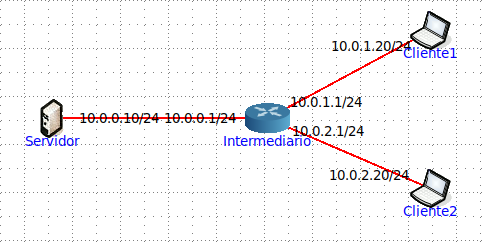
\includegraphics[width=0.5\textwidth]{images/Testes e resultados/cenario1.png}}
    \caption {Cenário 1}
\end{figure}

Na figura seguinte podemos observar o momento após todos os nodos da topologia se terem conectado ao \textit{Bootstrapper}.

\begin{figure}[H]
    \centering
    \frame{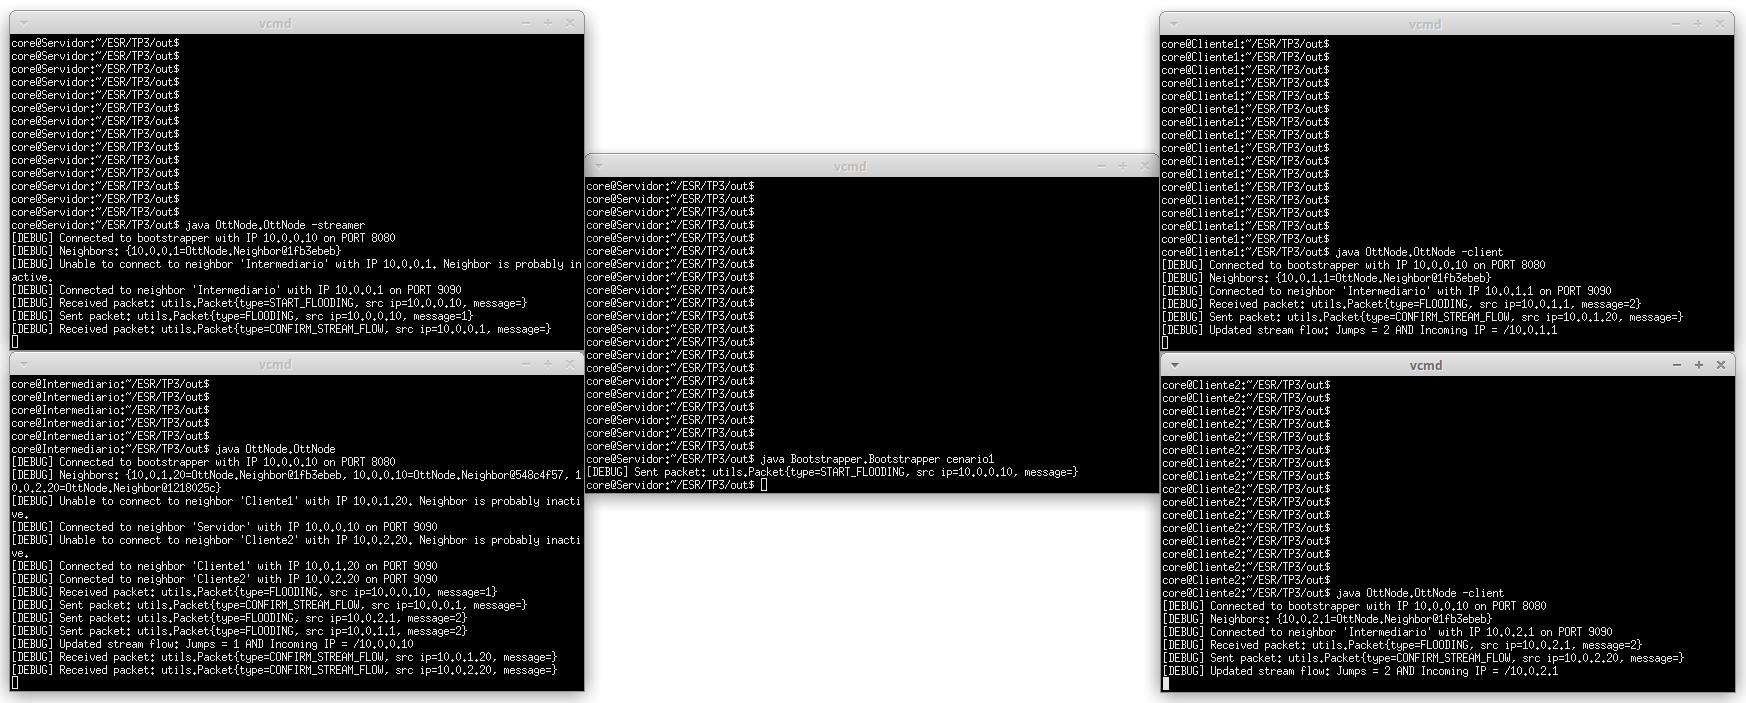
\includegraphics[width=1\textwidth]{images/Testes e resultados/cenario1_nodos_conectados.png}}
    \caption {Nodos conectados no cenário 1}
\end{figure}

Na figura seguinte podemos observar um cliente a consumir a \textit{stream}.

\begin{figure}[H]
    \centering
    \frame{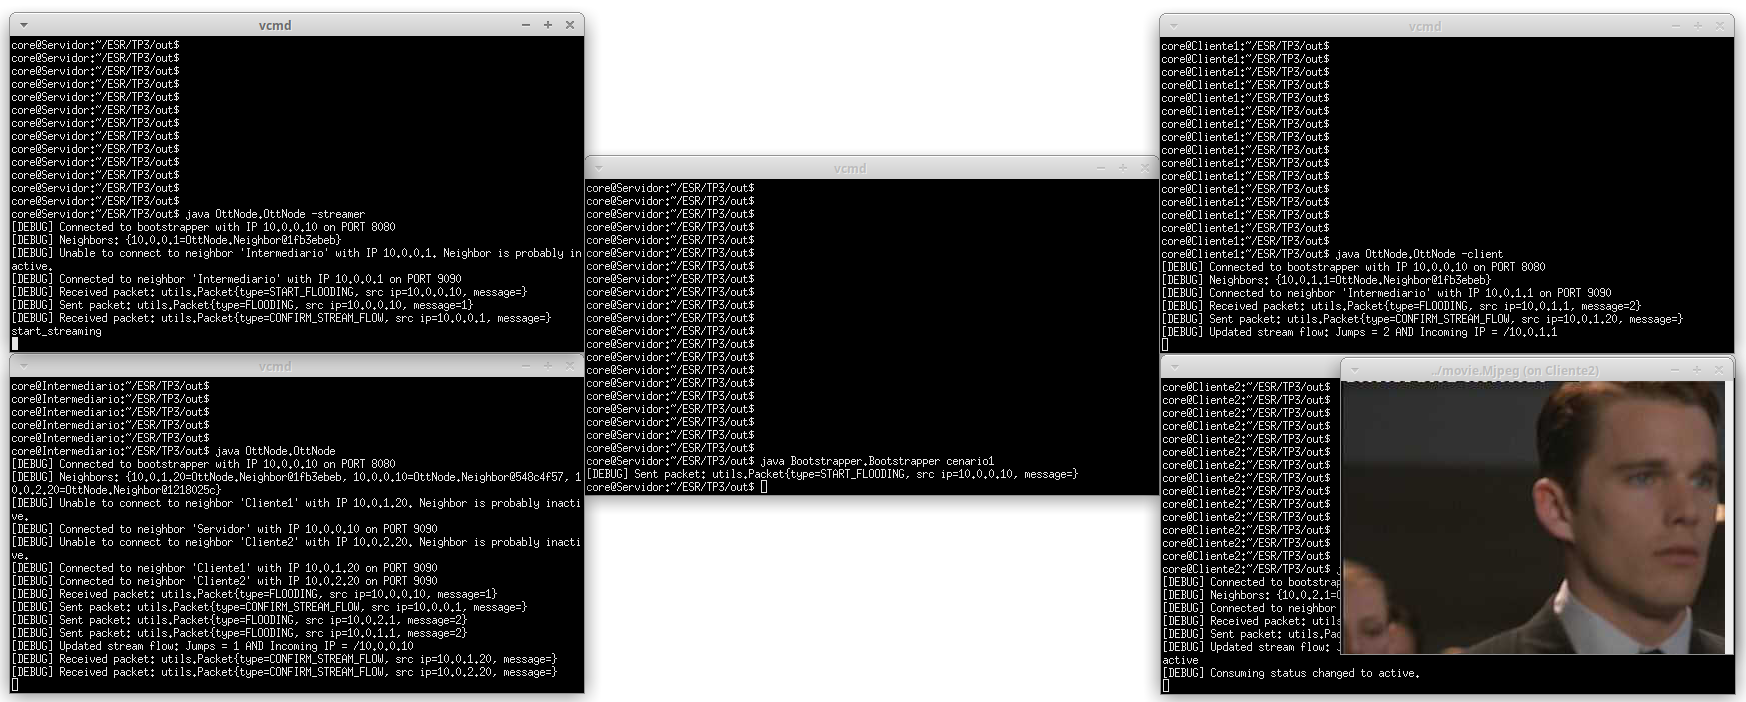
\includegraphics[width=1\textwidth]{images/Testes e resultados/cenario1_cliente2_consumindo_stream.png}}
    \caption {Cliente a consumir a \textit{stream} no cenário 1}
\end{figure}


\subsection{Cenário 2}

\begin{figure}[H]
    \centering
    \frame{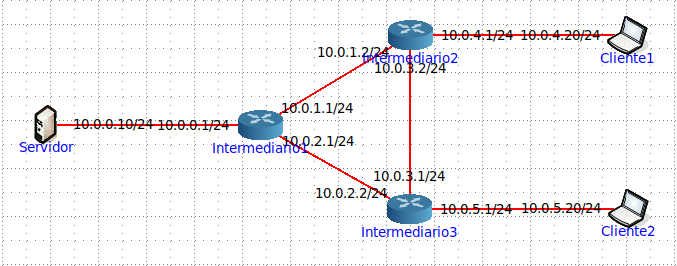
\includegraphics[width=.7\textwidth]{images/Testes e resultados/cenario2.png}}
    \caption {Cenário 2}
\end{figure}

Na figura seguinte podemos observar dois clientes a consumir a \textit{stream}.

\begin{figure}[H]
    \centering
    \frame{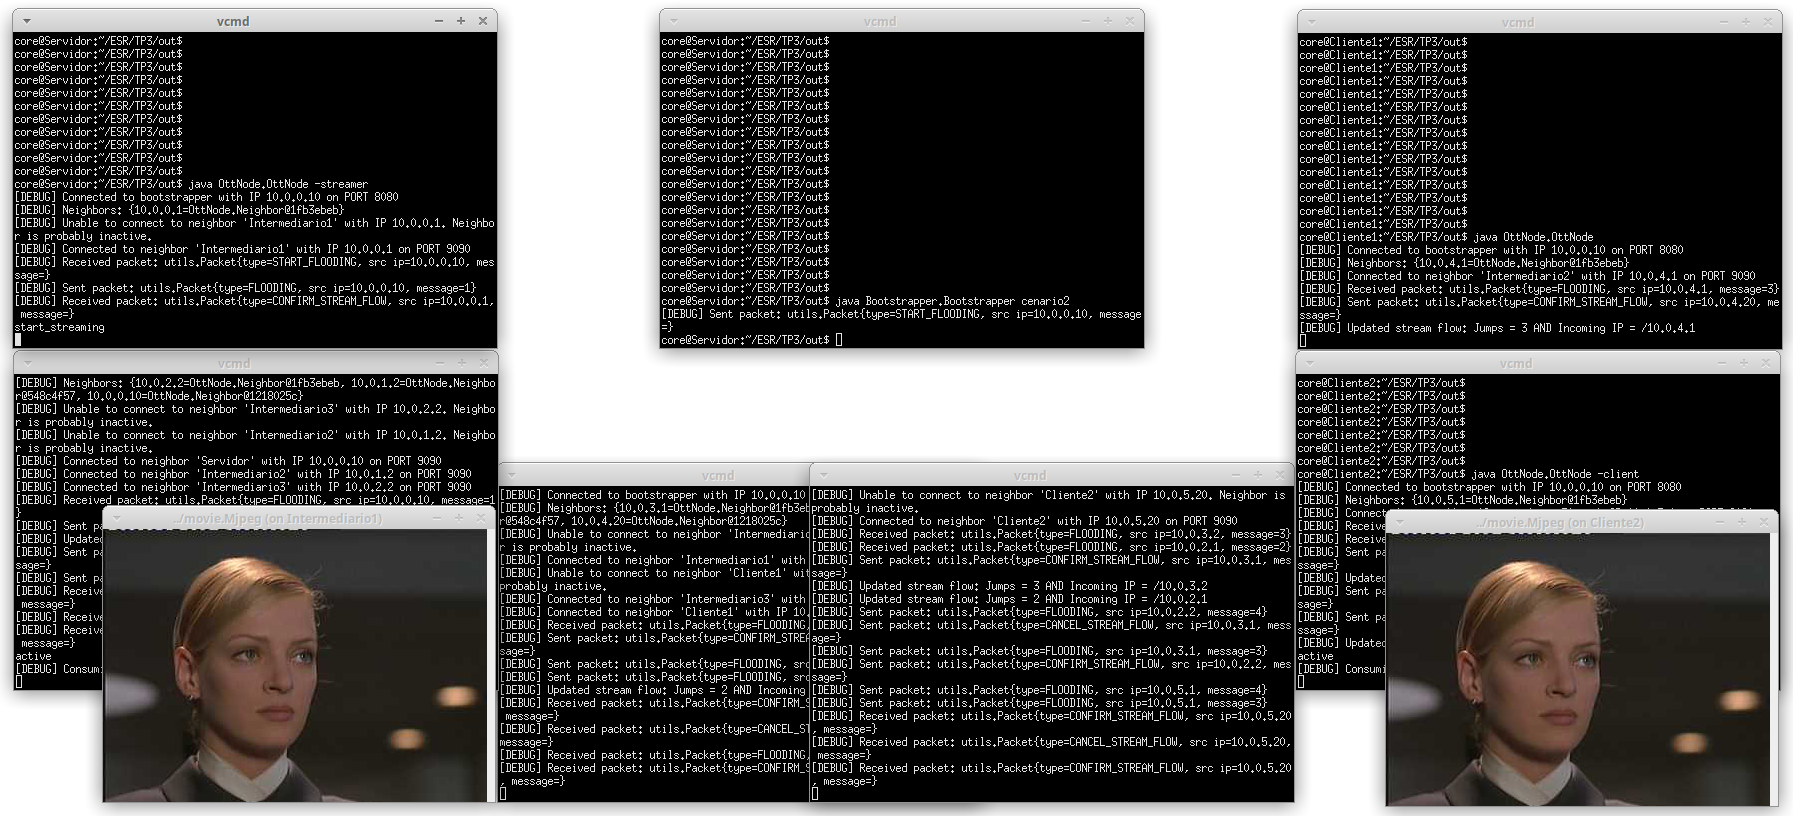
\includegraphics[width=1\textwidth]{images/Testes e resultados/cenario2_dois_clientes_consumindo.png}}
    \caption {Dois clientes a consumir a \textit{stream} no cenário 2}
\end{figure}


\subsection{Cenário 3}

\begin{figure}[H]
    \centering
    \frame{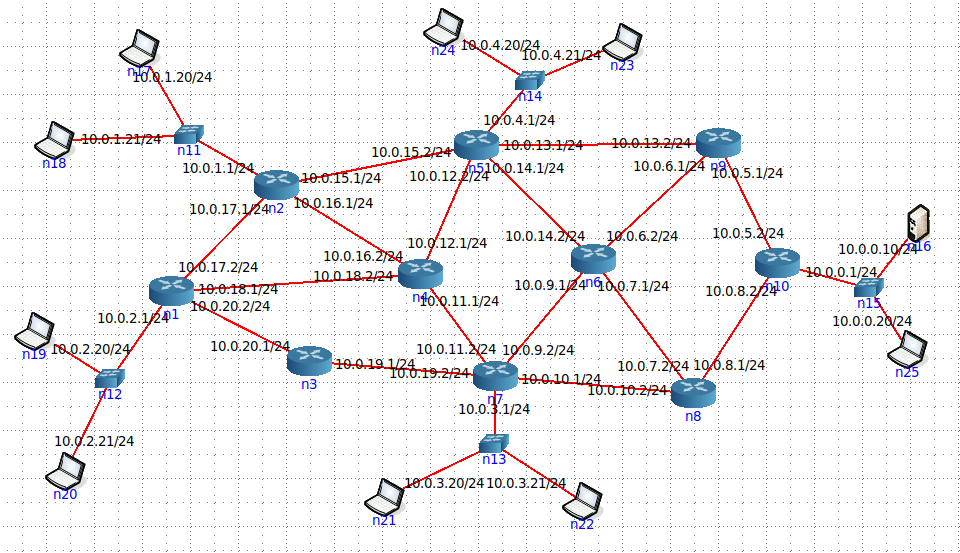
\includegraphics[width=.7\textwidth]{images/Testes e resultados/cenario3.png}}
    \caption {Cenário 3}
\end{figure}

Na figura seguinte podemos observar alguns clientes a consumir a \textit{stream}.

\begin{figure}[H]
    \centering
    \frame{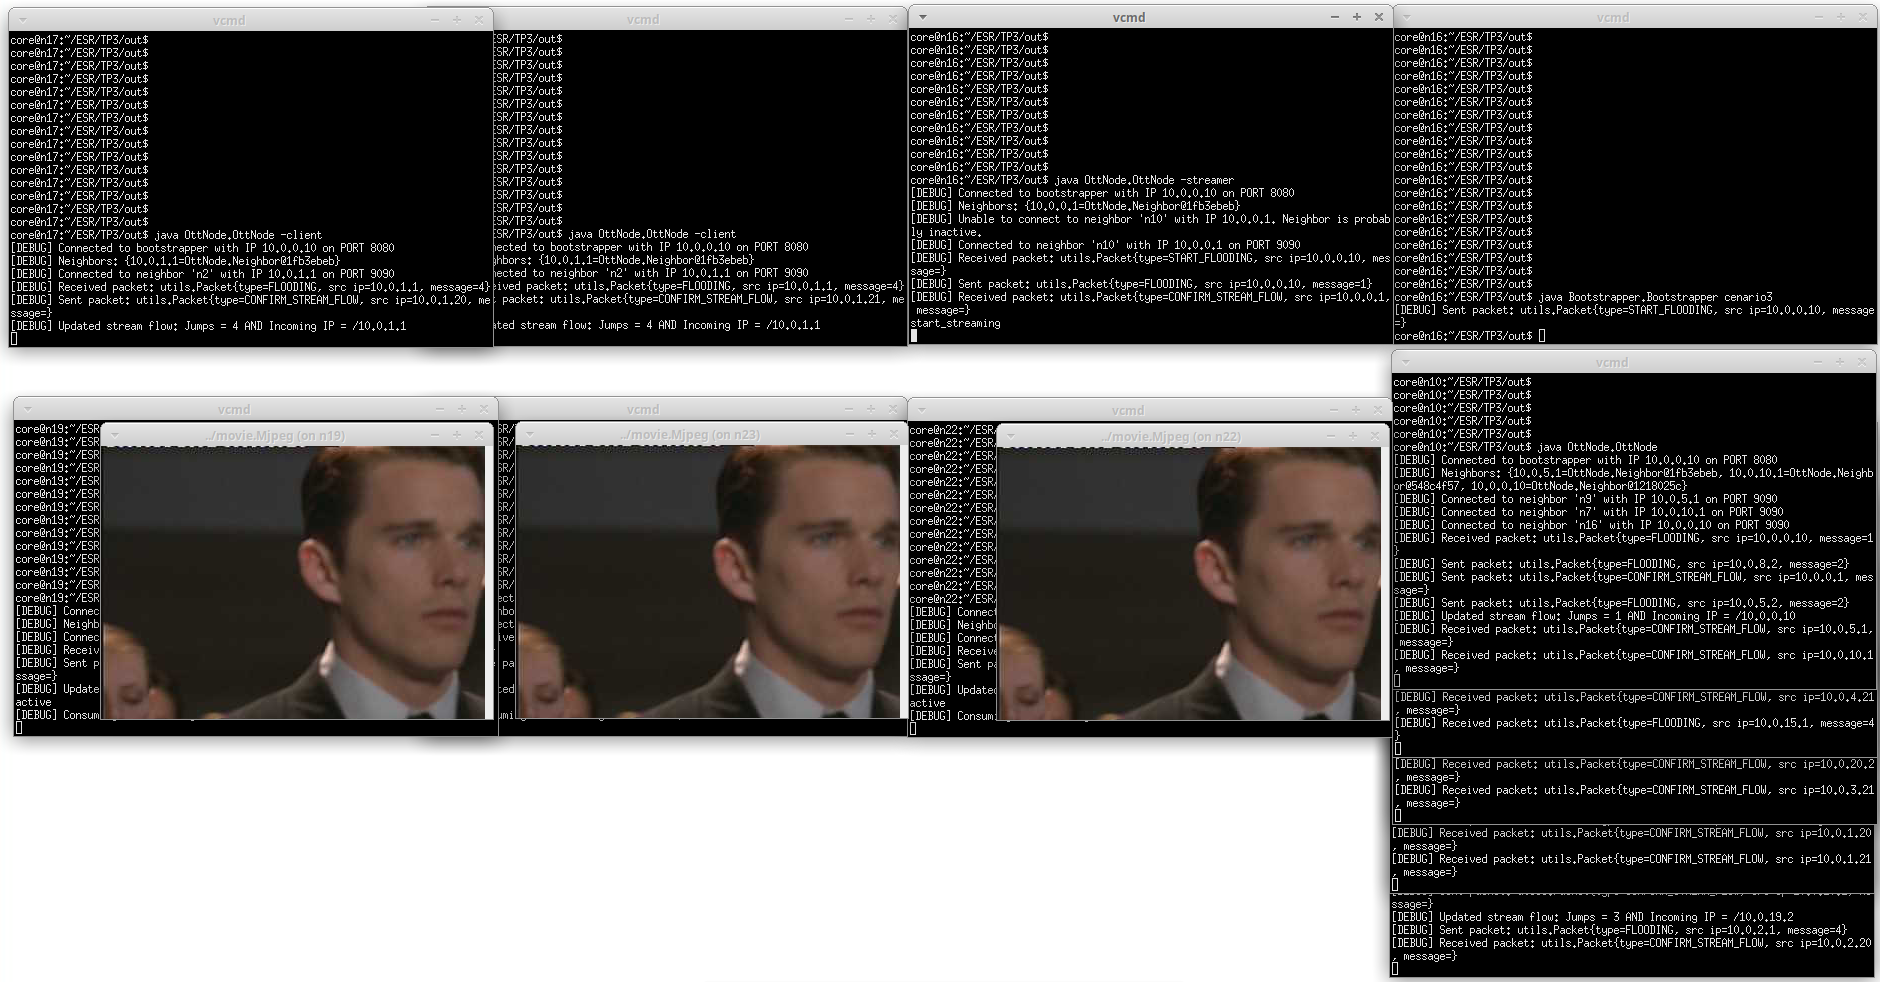
\includegraphics[width=1\textwidth]{images/Testes e resultados/cenario3_alguns_clientes_consumindo.png}}
    \caption {Alguns clientes a consumir a \textit{stream} no cenário 3}
\end{figure}

%-----------------------------------------------------------%


\section{Conclusão}

Em jeito de conclusão, o grupo sente-se satisfeito com o resultado final obtido e também em ter conseguido ultrapassar vários obstáculos com que se deparou ao longo do projeto. Ademais, pensamos que os objetivos principais do trabalho prático propostos pelos docentes da unidade curricular de Engenharia de Serviços em Rede foram atingidos com sucesso, uma vez que conseguimos pôr em prática os conhecimentos obtidos nas aulas e ainda aqueles que aprendemos de forma autodidata. Deste modo, fomos capazes de desenvolver um Serviço \textit{Over The Top} para efeitos de \textit{streaming} de vídeo em tempo real através de conexões TCP e UDP.


\clearpage
\begin{thebibliography}{}


% pergunta 1
\bibitem{ott}
\url{https://repositorio-aberto.up.pt/bitstream/10216/106138/2/203502.pdf}


\end{thebibliography}

\end{document}
